\chapter{Marco teórico}
% \section{Theoretical Framework}

% \subsection{Architecture of an ASR}

% Traditional architectures of an ASR are composed by 4 elements as illustrated on Figure \ref{fig:architecture}: a Signal Processing and Feature Extraction (FE), an Acoustic Model (AM) a Language Model (LM) and a Hypothesis Search.

% \begin{figure}
% \centering
% \begin{tikzpicture}[
% squarednode/.style={rectangle, draw=black!60, fill=white!5, very thick, minimum size=5mm},
% ]
% %Nodes
% \node[squarednode]      (am)                              {Acoustic model};
% \node[squarednode]        (fe)       [above=of am] {Feature Extraction};
% \node[squarednode]        (wave)       [above=of fe] {Audio Signal};
% \node[squarednode]      (hypothesis)       [right=2cm of am] {Hypothesis Search};
% \node[squarednode]        (lm)       [below=of hypothesis] {Language Model};
% \node[squarednode]        (result)       [above=of hypothesis] {Recognition Result};
 
% %Lines
% \draw[->] (wave.south) -- (fe.north);
% \draw[->] (fe.south) -- node{Feature}(am.north);
% \draw[->] (am.east) -- node{AM Score}(hypothesis.west);
% \draw[->] (lm.north) -- node{LM Score}(hypothesis.south);
% \draw[->] (hypothesis.north) -- (result.south);
% \end{tikzpicture}

% \caption{Classic architecture of an ASR \cite{Yu_2014_1}}
% \label{fig:architecture}
% \end{figure}

% The Feature Extraction (FE) process is usually called Front End because is the first step of Speech Recognition, its labor is to enhance the speech, removing distortions noise and transforming the wave in a representation that can be used from the Acoustic Model (AM), the AM estimates the probability for the transformed audio input given a known context and returns a score for the variable-length, the Language Model (LM) estimates the probability of a hypothesized word sequence; this approach uses N-grams with a very large collection of text, finally the Hypothesis Search merges the output of the AM and the LM. 
% Forced Alignment (FA) can be used inside the AM before begin the model training as used for CMU Sphinx \cite{Lee1990AnSystem}

Alineamiento Forzado (Forced Alignment FA) es un conjunto de técnicas para identificar los intervalos de tiempo entre los cuales una unidad de habla ocurre.
% Forced Alignment is a set of techniques to identify time intervals where speech units occur in transcribed speech. 

Para el análisis del habla, una unidad de habla es el segmento más pequeño en el cual está dividida la anotación de una señal; esta puede ser a nivel de declaración, la cual se define como el espacio de sonidos entre dos silencios, palabras o fonemas. Para el reconocimiento automático de la voz (Automatic Speech Recognition ASR), se usa generalmente una declaración para el entrenamiento y prueba de los algoritmos, sin embargo para el proceso de alineación forzada, se usa el nivel de fonemas.
% For speech analysis, a speech unit can be utterances, the speech audio between two silences, words or phonemes. Automatic Speech Recognition (ASR) generally uses utterance for its algorithms, however FA require a more fine grained annotation, usually at phoneme level.

\begin{figure}[H]

\centering
\caption{Alineación de una señal hablada}
\label{img:alignment}
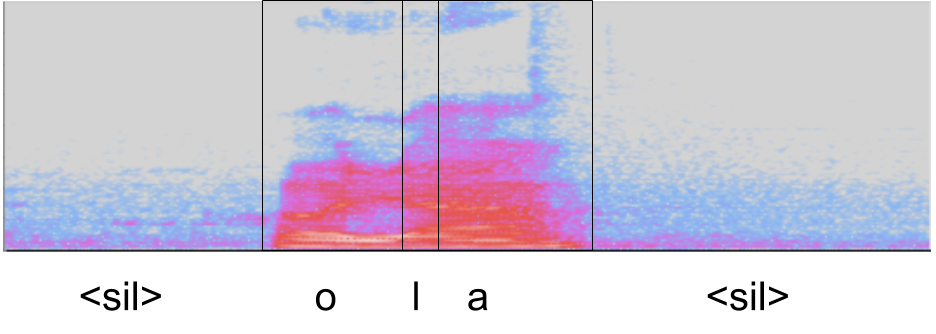
\includegraphics[scale=0.50]{images/alignment.png}
\end{figure}

En la figura \ref{img:alignment} se muestra un espectrograma de frecuencia que representa una señal hablada de la palabra Hola, bajo ella, una alineación fonética.

\section{Representación fonética}

Desde 1888, el Alfabeto Fonético Internacional (International Phonetic Alphabet IPA) es el métido estándar para representar y clasificar fonemas, indicando con un alto nivel de precisión las variaciones en la manera de articulación o la localización vocal de las modulaciones. Pequeñas variaciones en los fonemas son llamadas alófonos y pueden aumentar el nivel de anotación  \cite{IPAAlphabet}, pero en la práctica no son usados.
% Since 1888 the International Phonetic Alphabet (IPA) is the standard method to represent and classify phonemes, indicating with a high level of precision small variations of the manner of articulation or location of vocal tract modulations. Little variations on phonemes are called allophones and can improve the level of annotation \cite{IPAAlphabet}, but is not used in practice.

Las vocales son caracterizadas por la posición de la lengua y el tamaño de la abertura de la boca, teniendo diferentes representaciones, que se pueden observar en la tabla \ref{tab:ipa_table_vowels}. 
% Vowels are characterized by the position of the tongue and the wideness of the mouth having different representations variating the position as shown in Table \ref{tab:ipa_table_vowels}. 

Las consonantes están clasificadas en dos segmentos: las pulmónicas, que requieren aire saliendo de los pulmónes y las no pulmónicas, donde no sale aire. En ambas las modificaciones en el tracto bucal definen el sonido. Las consonantes están divididas en dentales, coronales, dorsales y laríngeas, las cuales a su vez están subdivididas en otros sub segmentos. También la manera de articular define el sonido producido, siendo las maneras de articular: plosivas, nasales, oclusivas, fricativas, aproximantes, eyectivas o implosivas.

Vea la clasificación de las consonantes en las tablas \ref{tab:ipa_table_pulmonic_consonants} y \ref{tab:ipa_table_non_pulmonic_consonants}.
% Consonants are classified in pulmonic and non-pulmonic, where modifications on superior vocal tract define the sound. All consonants are segmented in labial which subdivides in bi-labial labio-dental and labio-lingual; coronal divided into dental, alveolar, post-alveolar and retroflex; dorsal divided into palatal, velar, uvular; and laryngeal, divided in  pharyngeal and glottal; each classification can have a relationship with an articulation manner which is plosive, nasal, thrill, tap, flap, fricative, approximant, ejective, click or implosives. 

La representación del Alfabeto Fonético Internacional para las vocales está mostrado en la tabla \ref{tab:ipa_table_vowels}, donde se clasifican los sonidos por su centro silábico y la apertura del tracto bucal.
% IPA representation for vowels are mentioned in table \ref{tab:ipa_table_vowels}, pulmonic consonants are mentioned on table \ref{tab:ipa_table_pulmonic_consonants} and non-pulmonic consonants are mentiones on table \ref{tab:ipa_table_non_pulmonic_consonants}


\begin{landscape}
\begin{table}
\centering
\caption{Alfabeto Fonético Internacional: Consonantes pulmónicas}
\label{tab:ipa_table_pulmonic_consonants}
\begin{tabular}{|p{25mm}|l|p{15mm}|l|l|p{15mm}|l|l|l|l|l|l|}
\hline
{} & Bilabial & Labio\newline dental & Dental & Alveolar & Post-\newline alveolar & Retrofleja & Palatal & Velar & Uvular & Faríngea & Glotal \\
\hline
Plosiva& p b  & & \multicolumn{3}{|c|}{t d} & \textipa{\:t \:d } & \textipa{c \*j} & k g &  q G & & \textipa{P} \\
\hline
Nasal& m &  \textipa{M} & \multicolumn{3}{|c|}{n} & \textipa{\:n}  &  \textipa{\*n}  & \textipa{N} & N &  & \\
\hline
Vibrante& B & & \multicolumn{3}{|c|}{r}  & & & & R &  & \\
\hline
Aproximante & & \textipa{ⱱ} & \multicolumn{3}{|c|}{\textipa{R}} & \textipa{\:r} & & & & &  \\
\hline
Fricativa  & \textipa{F B}& f v & \textipa{T D} & s z & \textipa{S z} & \textipa{\:s \:z} & \textipa{\c{c} J}& x \textipa{G} &\textipa{X  K}  &\textcrh \textipa{Q} & h\textipa{H}  \\
\hline
Lateral \newline fricative& & & \multicolumn{3}{|c|}{\textbeltl \textipa{\*z}} & & & & &  & \\
\hline
Aproximante & & \textipa{V}& \multicolumn{3}{|c|}{\textipa{\!R}} & \textipa{\:R} & j  & \textturnmrleg & & &  \\
\hline
Aproximante lateral& & \multicolumn{3}{|c|}{\textipa{l}} &  \textraisevibyi & \textturny & \textipa{\;L} & & & & \\
\hline
\end{tabular}
\end{table}
\end{landscape}
% \begin{landscape}
\begin{table}
\centering
\caption{Alfabeto Fonético Internacional: Consonantes no pulmónicas}
\label{tab:ipa_table_non_pulmonic_consonants}
\begin{tabular}{|p{20mm}|l|l|l|l|l|l|}
\hline
{} & Bilabial & Dental & Alveolar  & Palatal & Velar & Uvular   \\
\hline
Eyectiva \newline oclusiva& p\textipa{'}  & &t   & c\textipa{'} & k\textipa{'} &  q\textipa{'}  \\
\hline
Eyectiva \newline fricativa& \textipa{F'}  & \textipa{T'}&  s\textipa{'} & \textipa{\c{c}'} & x\textipa{'} & \textipa{X'}  \\
\hline
Click &\textipa{\!o}  & \textipa{|} & \textipa{!} &  & & \\
\hline
Implosiva & \textipa{\!b}  & \multicolumn{2}{|c|}{\textipa{\!d}} &  \textipa{\!j} & \textipa{\!g} & \textipa{\!G} \\
\hline
\end{tabular}
\end{table}
% \end{landscape}
% \begin{landscape}
\begin{table}
\centering
\caption{Alfabeto Fonético Internacional: Vocales}
\label{tab:ipa_table_vowels}
\begin{tabular}{|l|l|l|l|l|l|l|}
\hline
{} & \multicolumn{2}{|c|}{Front} & \multicolumn{2}{|c|}{Central} & \multicolumn{2}{|c|}{Back}   \\
\hline
Cerrada & i  & y &\textbaru   & \textbari & \textturnm &  u  \\
\hline
Casi cerrada & \textsci  & \textscy &  \multicolumn{2}{|c|}{} &  & \textupsilon  \\
\hline
Semicerrada & e  & \textipa{\o} &\textreve &  \textbaro & \textramshorns & o \\
\hline
Intermedia &  \multicolumn{2}{|c|}{} & \multicolumn{2}{|c|}{\textschwa} &  \multicolumn{2}{|c|}{} \\
\hline
Semiabierta &\textepsilon  & \textipa{\oe} & \textrevepsilon & \textcloserevepsilon  & \textturnv & \textopeno \\
\hline
Casi abierta & \multicolumn{2}{|c|}{\ae} &\multicolumn{2}{|c|}{\textturna} &  \multicolumn{2}{|c|}{}  \\
\hline
Abierta & a  & \textscoelig &  \multicolumn{2}{|c|}{}  &\textscripta & \textturnscripta \\
\hline
\end{tabular}
\end{table}
% \end{landscape}

Cada idioma utiliza un subconjunto de los fonemas definidos en este alfabeto fonético.
% Each language uses a subset of phonemes to define its own pronunciation.

Cada palabra de cualquier idioma tiene una y solo una representación fonética, y la relación entre la palabra y esta representación es llamada diccionario fonético. Además de esta representación, son necesarias otras características para representar una señal hablada, como el silencio, los murmullos y otros sonidos que no representan palabras pero añaden información a la grabación del audio.
% Every language's word has only one phonetic representation and the relation between each word and its phonetic representation are called a phonetic dictionary. Besides the phonetic representation of each phoneme other features are needed to represent speech phenomenons like silence, mumbling and other inaudible sounds that can be perceived in a speech recording.

\section{Representación Digital}

Teniendo esta transcripción del audio, el resultado esperado de un Alineador Forzado es una lista de intervalos de tiempo relacionados a cada transcripción entre los cuales cada unidad fonética ocurre.
% Having the transcription of a speech audio the expected output from a FA is a list intervals where phonemes occurs.

Después de entender los principios fonológicos de la voz y su representación abstracta, se presenta una breve descripción de la representación computacional de las señales de voz.
% After understanding the phonological principles and its computational representation, an audio computational representation is also required.

Para representar una señal de voz analógica la manera más simple y aceptada es la Modulación por Impulsos Codificados (Pulse Code Modulation PCM) por la cual un transductor sensa la onda acústica correspondiente a la señal hablada en intervalos de tiempo uniformes y los traduce en una escala digital. La calidad de la representación digital depende de la frecuencia de muestreo (cantidad de muestras por segundo) y la profundidad de bits (cantidad de posibles valores digitales tomados en cada muestra). Con esta representación, un audio es solo una lista de valores en un rango determinado donde cada valor representa la presión de aire aplicada al transductor. Este formato es usualmente representado con extensiones .pcm, pero otros formatos de audio crudo son mayormente usados, como la extensión .wav, donde la misma secuencia de valores es almacenada y nombrada como canal, pero con prefijos que indican la frecuencia de muestreo, la profundidad de bits y otros valores específicos como la codificación de cada byte número de canales.
% To digitally represent an analog speech audio a widely accepted way is to use Pulse Code Modulation (PCM) where a transducer senses wave corresponding to the speech on a uniform time interval and translated it in a digital scale. The quality of the digital representation depends on the sampling rate (quantity of measurements by second) and the bit depth (possible digital values to represent each sample). With this representation, an audio is just a list of values in a range that varies representing the pressure applied to a transducer. This format is usually represented with a .pcm extension, but other formats of raw audio exists, like .wav, where the raw audio is stored after a set of headers that defines sampling rate, bit depth, endianness and number of channels.

La representación cruda del audio es útil para reconstruir la señal análoga de una manera mas sencilla, pero para entender la relación entre esta señal digital y su representación fonética es necesario recurrir a técnicas para el procesamiento digital de señales.
% Raw representation of audio is useful to reconstruct easily the analog signal, but to understand the relation between audio segments and phonetic information new ways to represent audio needs to be define.

\section{Técnicas de alineamiento}

Para tener una manera uniforme de representar cada audio, el análisis de frecuencias en cortos periodos de tiempo (Short Time-Frequency Analysis), es una técnica muy usada, la cual consiste en dividir la señal en segmentos uniformes y desfasados en una unidad constante menor a la del tamaño del segmento, buscando que cada segmento se comporte como una señal estacionaria con la cual se pueden extraer parámetros de frecuencia usando transformadas como Fourier o Wavelet, una ilustración de este proceso puede observarse . Esta fase del análisis es conocida como Extracción de Características (Feature Extraction FE) y se usan técnicas como Mel Frequency Cepstral Coefficients (MFCC)\cite{Davis1980ComparisonSentences}, Perceptual Linear Prediction (PLP) \cite{Hermansky1990PerceptualSpeech}, Linear frequency cepstral coefficients LFCC \cite{Davis1980ComparisonSentences}, Wavelet-packet features (WPF) \cite{Farooq2001MelRecognition}, Subband-based cepstral parameters (SBC) \cite{Sarikaya98waveletpacket}, Mixed wavelet packet advanced combinational encoder (MWP-ACE) \cite{NogueiraWaveletImplants} entre otras.

\begin{figure}[H]

\centering
\caption{Extracción de características}
\label{img:fe}
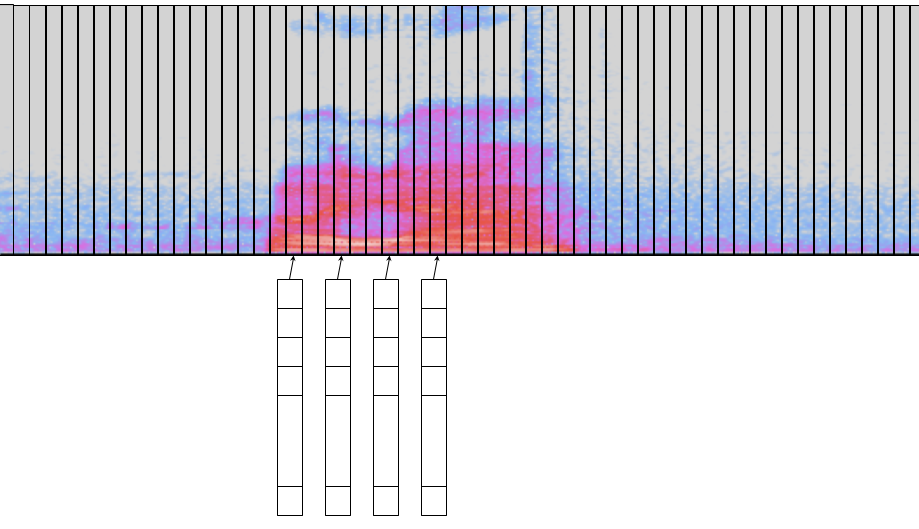
\includegraphics[scale=0.50]{images/fe.png}
\end{figure}

En la figura \ref{img:fe} se muestra un esquema de extracción de características usando un desfase igual al tamaño de la ventana de tiempo de cada segmento. De cada ventana de tiempo se extraen características de la señal que en ese segmento se comporta como una señal estacionaria.
% To have a more uniform way to represent each audio, short time-frequency analysis are used and the technique consists in split the audio in fixed length chunks and each chunk with a defined offset usually less than the chunk length itself, and extract frequency features of each chunk using transforms like Fourier or Wavelet, this phase is usually called Feature Extraction and techniques like Mel Frequency Cepstral Coefficients (MFCC)\cite{Davis1980ComparisonSentences}, Perceptual Linear Prediction (PLP) \cite{Hermansky1990PerceptualSpeech}, Linear frequency cepstral coefficients LFCC \cite{Davis1980ComparisonSentences}, Wavelet-packet features (WPF) \cite{Farooq2001MelRecognition}, Subband-based cepstral parameters (SBC) \cite{Sarikaya98waveletpacket}, Mixed wavelet packet advanced combinational encoder (MWP-ACE) \cite{NogueiraWaveletImplants}.

Con esta nueva representación discreta de la señal hablada, un modelo que identifique los límites entre fonemas suele ser mas claro, pues existe similaridad entre cada segmento de la fase anterior.
% With this new representation a model to identify intervals and boundaries between phonemes are clear, because similar 

Para crear un modelo de alineación de audio las aproximaciones se dividen en 3 grupos: Pliegue Dinámico Temporal (Dynamic Time Warping DTW)  \cite{Sakoe1978DynamicRecognition}, en donde se generan artificialmente señales equivalentes a las esperadas en la señal de audio con la descripción fonética de la misma y luego se calcula una matriz de diferencias entre las señales, buscando valores intermedios que minimicen la diferencia entre ambas señales. La segunda aproximación utiliza Modelos Ocultos de Markov (Hidden Markov Models HMM) los cuales determinan un modelo probabilístico de transición entre fonemas a partir de datos propiamente anotados para posteriormente con este modelo definir la nueva alineación de las señales propuestas \cite{RabinerARecognition}. La última aproximación utiliza Redes Neuronales Artificiales (Artificial Neural Networks ANN) homogenizando la señal en secuencias de vectores y creando modelos que maximicen la predicción de los fonemas esperados  \cite{Deng2012}.

A continuación se describen las tres técnicas más usadas para realizar alineación forzada:
% To create a model to align speech three major techniques are used, the first is called Dynamic Time Warping (DTW) \cite{Sakoe1978DynamicRecognition} where an artificial wave with the phonetic representation of the annotation is created and then an alignment algorithm minimize the difference using a distance matrix. Another widely used approach is to use HMM where a probabilistic model is created to represent the transition between phonemes and then use this model to align existing waves \cite{RabinerARecognition}. The last approach is ANN using a normalization model to homogenize speech in sequences of vectors and create a model that maximize the prediction of a new vector \cite{Deng2012}.

\subsection{Pliegues Dinámicos Temporales}

Para el DTW la idea principal es eliminar la fluctuación de una señal particular con respecto a una generada sintéticamente creando una normalización temporal donde los fonemas correspondientes ocurren en intervalos te tiempo recurrentes. Para lograr esta normalización, se utilizan algoritmos de programación dinámica para maximizar la coincidencia entre dos patrones de voz. Las transformaciones en el tiempo que se hacen hacen  en ambas señales, son llamadas aproximaciones simétricas y se espera una función objetivo que minimice la distancia entre las dos señales.
% For DTW the main idea es to eliminate the fluctuation of a particular speech creating a time normalization where phonemes occur in a recurrent time interval. To achieve this normalization, dynamic programming algorithms are proposed to generate the maximum coincidence between two speech patterns. Time speech transformations are usually made in both signals, this is called a symmetric approach, and a function that minimizes the distance between both signals is the expected output. 

\begin{figure}[H]

\centering
\caption{Pliegues Dinámicos Temporales \cite{Zhang2017DynamicLength}}
\label{img:dtw}
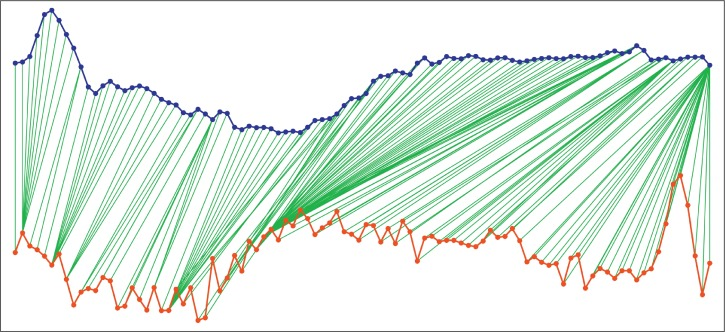
\includegraphics[scale=0.50]{images/dtw.jpg}
\end{figure}

En la figura \ref{img:dtw} se muestra un proceso de pliegue dinámico unidireccional de la señal representada por los puntos rojos a la señal con representada con los puntos verdes.

Generar una señal artificial a partir de la representación fonética de la señal deseada requiere un conocimiento previo de la equivalencia fonética-acústica teniendo modelos basados en reglas que se concatenan para generar la señal objetivo. El proceso de generación de señales acústicas a partir de representaciones fonéticas es llamado Texto a Voz (Text To Speech TTS) y usualmente se obtiene como resultado inverso de un proceso de ASR donde se utiliza el modelo de conocimiento como modelo de generación.
% Generating an artificial wave with the phonetic representation of real speech, where the algorithm know a priori the intervals where each phoneme occurs and minimizing the distance between those two waves, a reconstruction of the real speech wave can be perform using the opposite sequence that minimize the distance between the waves.

\subsection{Modelos Ocultos de Markov}

Alinear una onda usando Modelos Ocultos de Markov requiere un modelo pre existente que defina los estados ocultos de cada modelo de Markov. Esta estimación inicial se realiza por medio del algoritmo Baum-Welch \cite{RabinerARecognition} el cual define unos valores iniciales que pueden ser aleatorios y los modifica en cada iteración hasta tener una configuración apropiada para las etiquetas y los estados usando un algoritmo de maximización de expectativa (Expectation Maximation EM). La generación de este modelo permite definir una matriz de costos que se puede optimizar por medio del algoritmo de Viterbi para encontrar la secuencia de etiquetas más probable para la entrada data. En el caso de las señales habladas, la entrada está representada por una secuencia de vectores con características de cada ventana de señal y la salida es su correspondiente secuencia de fonemas.
% Aligning a wave using HMMs requires a preexisting model that defines the hidden states of the markov models. This estimation usually uses a Baum-Welch algorithm, where a set of values are proposed for the hidden layer usually randomly and maximized using an Expectation-Maximization algorithm. This model then allows to use the Viterbi algorithm to find a maximum sequence of probability of hidden states for a new sequence, where the sequence is a speech vector and the hidden state represents the phonemes.

\begin{figure}[H]

\centering
\caption{Modelos Ocultos de Markov}
\label{img:hmm}
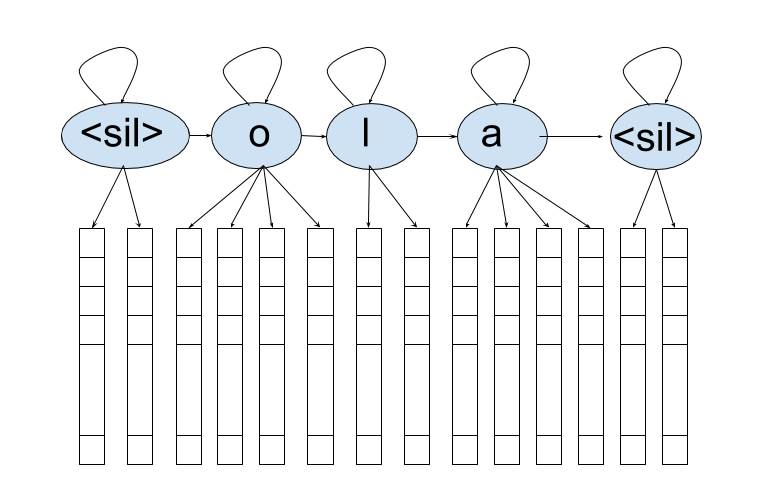
\includegraphics[scale=0.50]{images/hmm.png}
\end{figure}

En la figura \ref{img:hmm} se muestra una posible configuración de estados que representan fonemas y la secuencia de vectores extraídos de la señal hablada

\subsection{Redes Neuronales Artificiales}

Las implementaciones de redes neuronales artificiales para enfrentar el problema de la identificación de secuencias de fonemas a partir de señales habladas es muy variada, existiendo aproximaciones fin-a-fin (End to End) donde se toma directamente la señal cuantizada y por medio de topologías profundas se obtienen modelos aproximados \cite{Hannun2014}. Otras aproximaciones usan algoritmos los extracción de características mencionados anteriormente y en vez de usar los algoritmos de Baum-Welch  para parametrizar los Modelos Ocultos de Markov utilizan redes neuronales, en un esquema similar al mostrado en la imagen \ref{img:cd-dnn-hmm}
% ANN approaches uses vectorization to homogenize speech data and generates a network topology that minimize the error of a new vector.

\begin{figure}[H]

\centering
\caption{Redes Neuronales y Modelos de Markov \cite{Deng2012}}
\label{img:cd-dnn-hmm}
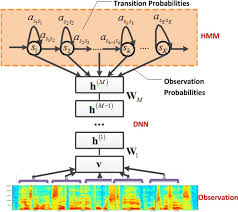
\includegraphics[]{images/cd-dnn-hmm.jpeg}
\end{figure}


